\documentclass{beamer}
\usepackage[spanish]{babel}
\usepackage{ragged2e}
\usepackage{listings}

\addtobeamertemplate{block begin}{}{\justifying}{}
\apptocmd{\frame}{}{\justifying}{}


\title{Modelado y simulación del Robot Mitsubishi RV-2JA controlado
mediante señales electromiográficas}

\author{
    Busso, Francisco Ignacio \and
    \\ Gautero, Francisco \and
    \\ Gregoret, Guillermo}
\institute{Universidad Tecnológica Nacional\\Facultad Regional Santa Fe}
\date{\today}



\begin{document}

    \begin{frame}
        \titlepage
    \end{frame}

    \begin{frame}
        \frametitle{Objetivo}
        \hspace*{20pt}Controlar al Robot Mitsubishi RV-2JA mediante señales electromiográficas de superficie sEMG.
        \begin{figure}
            \centering
            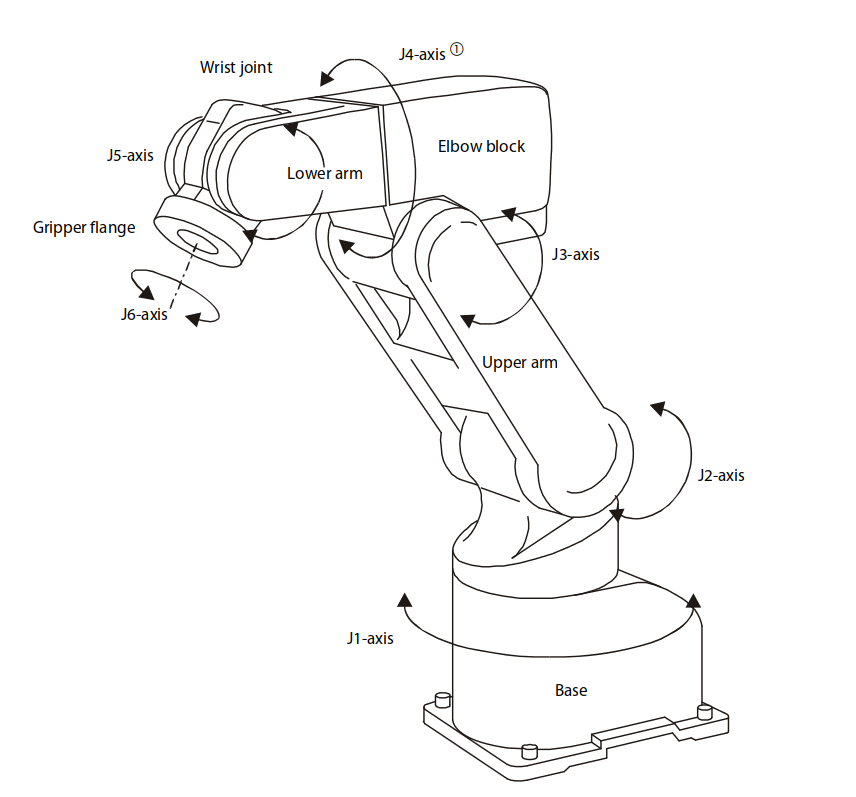
\includegraphics[scale=0.2]{robot.png}
            \caption{Robot Mitsubishi RV-2JA}
        \end{figure}
    \end{frame} 

    \begin{frame}
        \frametitle{Etapas del Trabajo}
        El trabajo original se divide en 3 aspectos principales:
            \begin{enumerate}
             \item Lectura y análisis de señales.
             \item Reconocimiento de patrones a través de RNA.
             \item Interfaz electrónica simulada.
            \end{enumerate}
    \end{frame} 

    \begin{frame}
        \frametitle{Funcionamiento del Robot}
        \hspace*{20pt}El sistema electromiográfico está diseñado para que el operador controle al robot de forma remota; 
        las señales sEMG son tomadas del operador y pertenecen a movimientos musculares específicos, estas son procesadas en 
        el programa encargado de extraer sus características particulares para determinar el tipo de movimiento que realizará 
        el robot.\\~\
        
        \hspace*{20pt}Las características identificadas de las señales sEMG ingresan a una red neuronal artificial que activa las 
        correspondientes articulaciones del robot que se desee mover con determinada posición de la mano.
    \end{frame} 

    \begin{frame}
        \frametitle{Obtención de los Datos de Entrada}
        \hspace*{20pt}En el desarrollo del paper se utilizó el brazalete Myo como dispositivo de entrada para la adquisición de datos. 
        Los datos de entrada son analizados mediante el diseño de un programa en Matlab-Simulink que proporciona datos de 
        entrenamiento para las redes neuronales del sistema.\\~\
        
        \hspace*{20pt}En un entorno virtual se realiza una simulación detallada del robot la cual permitirá 
        replicar los movimientos deseados por el operador para luego validar los resultados del procesamiento y entrenamiento 
        del sistema. 
    \end{frame}
    
    \begin{frame}
        \frametitle{Modelo Simulink}
        \begin{figure}
            \centering
            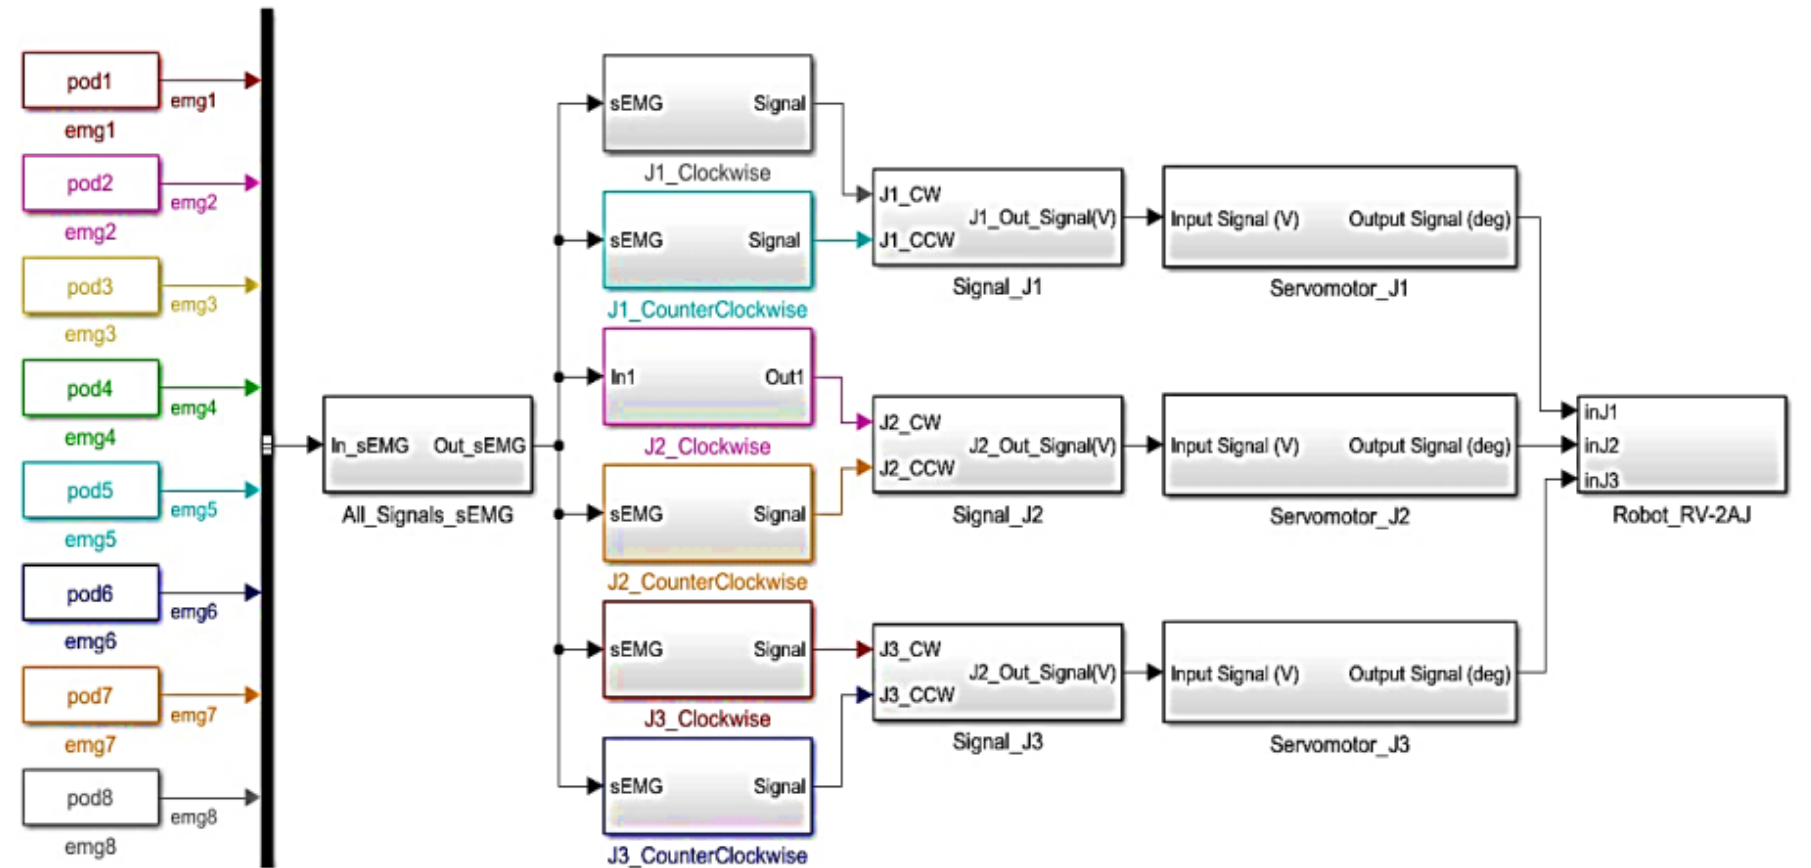
\includegraphics[scale=0.23]{simulink-model.png}
            \caption{Arquitectura del modelo diseñado en Simulink.}
        \end{figure}
    \end{frame} 

    \begin{frame}
        \frametitle{Arquitectura de la Red Neuronal}
        \hspace*{20pt}Para la arquitectura de la red es necesario escoger el número de neuronas ocultas; con los parámetros seleccionados
         se procede al entrenamiento de la red usando un algoritmo de aprendizaje supervisado que se usa para entrenar redes neuronales 
         artificiales. Se aplica el modelo Backpropagation que es la propagación hacia atrás de errores o retropropagación.\\~\
        
        \hspace*{20pt}Cuando la red neuronal artificial ya está entrenada se generan versiones desplegables de la red neural entrenada.
        
    \end{frame} 

    \begin{frame}
        \frametitle{Arquitectura de la Red Neuronal}
        \begin{figure}
            \centering
            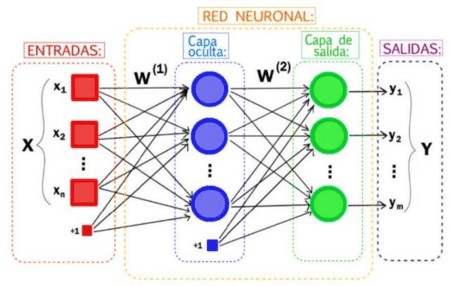
\includegraphics[scale=0.6]{network.jpg}
            \caption{Arquitectura de la Red Neuronal}
        \end{figure}
    \end{frame} 

    \begin{frame}
        \frametitle{Dificultades encontradas}
        \begin{enumerate}
            \item Resolución del análisis de señales.
            \item Obtención de un dataset.
        \end{enumerate}
    \end{frame} 

    \begin{frame}
        \frametitle{Nuestra Solución}
        \hspace*{20pt}Optamos por resolver una RNA capaz de detectar la posición FIST, ya que esta es la única que 
        ejemplifica sus datos en el paper.\\~\

        \hspace*{20pt}Tomamos los valores medios de cada lectura del sensor como valor original, 
        y en base a ellos generamos un dataset propio definiendo un valor arbitrario de tolerancia.
        
    \end{frame} 

    \begin{frame}
        \frametitle{Valores de Referencia}
        \begin{table}[]
            \resizebox{11cm}{!}{
                \begin{tabular}{|l|l|l|l|l|l|l|l|l|}
                    \hline
                                         & \textbf{emg1} & \textbf{emg2} & \textbf{em3} & \textbf{emg4} & \textbf{emg5} & \textbf{emg6} & \textbf{emg7} & \textbf{emg8} \\ \hline
                    \textbf{Valor Medio} & 0.0449        & 0.0385        & 0.0481       & 0.0628        & 0.0897        & 0.0982        & 0.0814        & 0.0833        \\ \hline
                    \textbf{IEMG}        & 0.5731        & 0.3816        & 0.1019       & 0.1996        & 0.7386        & 0.8177        & 1.1194        & 1.2671        \\ \hline
                    \textbf{MAV}         & 0.0179        & 0.0119        & 0.0032       & 0.0062        & 0.0231        & 0.0256        & 0.0350        & 0.0396        \\ \hline
                    \textbf{RMS}         & 0.0048        & 0.0035        & 0.0014       & 0.0026        & 0.0072        & 0.0082        & 0.0082        & 0.0097        \\ \hline
                    \textbf{VAR}         & 0.0031        & 0.0014        & 0.0001       & 0.0006        & 0.0036        & 0.0036        & 0.0094        & 0.0116        \\ \hline
                \end{tabular}
            }
            \caption{Características de la señal sEMG, posición de mano FIST.}
            \end{table}
    \end{frame} 

    \begin{frame}
        \frametitle{Valores de Referencia}
        \hspace*{20pt}Para generar valores de cada señal EMG se optó por una distribución uniforme con 
        variación del 5\% sobre las señales de referencia.
        \begin{figure}
            \centering
            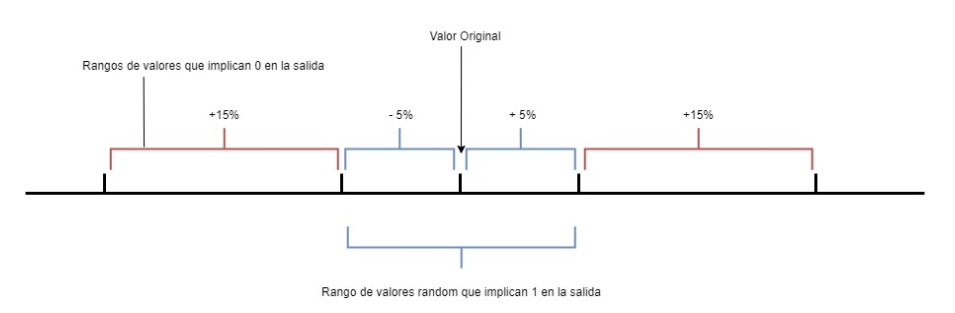
\includegraphics[scale=0.45]{grafico-pela.png}
        \end{figure}
    \end{frame} 

    \begin{frame}
        \frametitle{Valores de Referencia}
        \begin{figure}
            \centering
            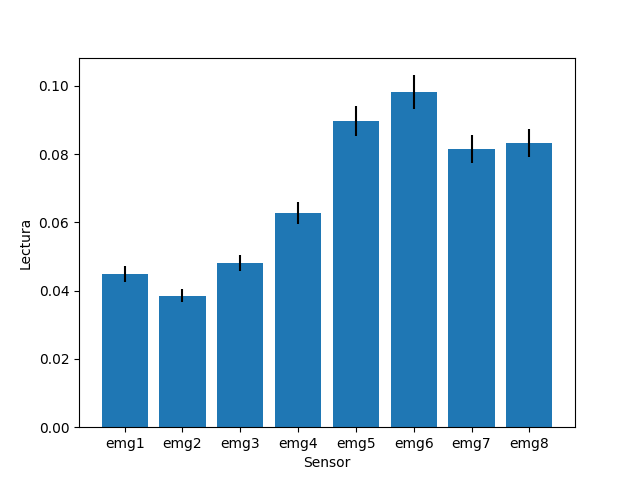
\includegraphics[scale=0.4]{plot.png}
            \caption{Valores de Referencia para cada sensor}
        \end{figure}
    \end{frame} 

    \begin{frame}
        \frametitle{Etiquetado del Set de Datos}
        \hspace*{20pt}Se define un valor umbral para determinar si el valor de la lectura de un sensor pertenece a los valores admitidos.
        \vspace*{5pt}
        \lstinputlisting[language=Python, firstline=1, lastline=3, basicstyle=\tiny]{snippets.txt}
        \vspace*{10pt}
        \hspace*{20pt}Si las lecturas de todos los sensores se encuentran dentro del rango admitido, la entrada se etiqueta como 1; si no, se etiqueta como 0.
        \vspace*{5pt}

        \resizebox{11cm}{!}{
            \lstinputlisting[language=Python, firstline=5, lastline=6]{snippets.txt}
        }
    \end{frame} 

    \begin{frame}
        \frametitle{Obtención del Set de Entrenamiento}
        \hspace*{20pt}Se lee un set de datos, se lo etiqueta y se lo separa entre un set de entrenamiento y un set de pruebas.
        \vspace*{10pt}

        \resizebox{11cm}{!}{
            \lstinputlisting[language=Python, firstline=8, lastline=16]{snippets.txt}
        }

    \end{frame}   


    \begin{frame}
        \frametitle{Implementación con scikit-learn}

        \hspace*{20pt}La clase MLPClassifier implementa un algoritmo de entrenamiento de perceptrón 
        multicapa \textit{(MLP)} utilizando propagación hacia atrás \textit{(Backpropagation)}.
        \vspace*{10pt}

        \resizebox{10cm}{!}{
            \lstinputlisting[language=Python, firstline=18, lastline=21]{snippets.txt}
        }



    \end{frame}

    \begin{frame}
        \frametitle{El Algoritmo MLP}
        \hspace*{20pt}El algoritmo toma como entrada dos arreglos: $X$, de dimensiones ($n-muestras$, $n-caracteristicas$), 
        que representa las muestras de entrenamiento como vectores de punto flotante; e $Y$ de tamaño ($n-muestras$), 
        que almacena los valores de las etiquetas de clase para las muestras de entrenamiento.
        \vspace*{10pt}

        \resizebox{10cm}{!}{
            \lstinputlisting[language=Python, firstline=23, lastline=26]{snippets.txt}
        }


    \end{frame}

    \begin{frame}
        \frametitle{Estrategia de Resolución: Algoritmo L-BFGS}

        \hspace*{20pt}Es un algoritmo de optimización de la familia de los métodos \textit{quasi-Newton} que aproxima al algoritmo 
        (\textit{BFGS}) utilizando una cantidad limitada de memoria. Es un algoritmo muy popular de estimación de parámetros en Machine Learning.\\~\

        \hspace*{20pt}Para cada iteración el algoritmo busca una aproximación de la inversa de la matriz Hessiana, almacenando solo unos pocos
        vectores que representan a la aproximación implícitamente

    \end{frame}

    \begin{frame}
        \frametitle{Función de activación: Rectificador}

        \hspace*{20pt}En el contexto de las redes neuronales artificiales, el rectificador es una función de activación definida 
        como:

        \begin{equation}
            ReLU(x) = x^+ = max(0, x)
        \end{equation}

        \hspace*{20pt}Donde $x$ es la entrada de la neurona. También es conocida como función rampa y es análoga a la rectificación de 
        media onda en electrónica.
    \end{frame}

    \begin{frame}
        \frametitle{Predicciones}

        \hspace*{20pt}Luego del ajuste (entrenamiento), el modelo puede predecir las etiquetas para nuevas muestras
        \vspace*{10pt}

        \resizebox{9cm}{!}{
            \lstinputlisting[language=Python, firstline=28, lastline=29]{snippets.txt}
        }

    \end{frame}

    \begin{frame}
        \frametitle{Cálculo de Error}

        \hspace*{20pt}Se calculó el error comparando la salida esperada con la salida obtenida por el clasificador.

        \begin{table}[]
            \begin{tabular}{|l|l|}
            \hline
            \textbf{Neuronas Ocultas} & \textbf{Error} \\ \hline
            5                         & 52.2\%         \\ \hline
            10                        & 24.1\%         \\ \hline
            15                        & 28.0\%         \\ \hline
            20                        & 0.0\%          \\ \hline
            \end{tabular}
            \caption{Numero de neuronas y error obtenido. Función de activación Rectificador.}
        \end{table}

    \end{frame}

    \begin{frame}
        \frametitle{Complejidad de la Solución}

        \hspace*{20pt}Suponiendo $n$ muestras de entrenamiento, $m$ características, $k$ capas ocultas cada una conteniendo $h$ 
        neuronas y, para simplificar, o neuronas en la capa de salida. La complejidad temporal de la propagación hacia atrás es 
        $O(n*m*h^k*o*i)$, donde $i$ es el número de iteraciones. \\~\
        
        \hspace*{20pt}Dado que el método de \text{Backpropagation} tiene alta complejidad temporal, es recomendable comenzar con un número 
        bajo de neuronas en la capa oculta para el entrenamiento.

    \end{frame}  

    \begin{frame}
        \frametitle{Conclusiones}

        \hspace*{20pt}Mediante el uso de una RNA MLP, entrenada con un algoritmo de backpropagation y datos creados artificialmente, 
        se pudo identificar el patrón que refiere a la posición de maño fist de manera que el resultado es estable y repetible.
    \end{frame}  

    \begin{frame}
        \frametitle{Conclusiones}
        \hspace*{20pt}Haciendo una comparación con los resultados originales en cuestión de error, no tuvimos como identificar la métrica observada ni 
        como fue calculada. No obstante propusimos una métrica adecuada y podemos ver una relación similar error/cantidad 

        
        \begin{table}[]
            \resizebox{11cm}{!}{
            \begin{tabular}{|l|l|l|}
            \hline
            \textbf{Cantidad de Neuronas Ocultas} & \textbf{Error Obtenido en el Paper} & \textbf{Error Calculado} \\ \hline
            5                                     & 4.39                                & 52.2\%                   \\ \hline
            10                                    & 4.29                                & 24.1\%                   \\ \hline
            15                                    & 4.44                                & 28.0\%                   \\ \hline
            20                                    & 4.29                                & 0.0\%                    \\ \hline
            \end{tabular}
            }
            \caption{Comparación del Error.}
            \end{table}
        
    \end{frame}  

    \begin{frame}
        \frametitle{Conclusiones: Escalabilidad de la Solución}

        \hspace*{20pt}Esta implementación no está pensada para aplicaciones de gran escala. 
        En particular, scikit-learn no ofrece soporte para GPU.
    \end{frame}  

    \begin{frame}
        \frametitle{Código Fuente}
        El código fuente puede ser consultado en \href{https://github.com/fbusso/ic-tp1}{\textit{GitHub}}
    \end{frame} 
\end{document}